%*********************************************************************
%	THERMAL SYSTEM IDENTIFICATION
%*********************************************************************
\chapter{Thermal System Identification}
\label{ch:thermalID}

Chapter~\ref{ch:theory} modelled both thermal loops from geometry and material properties. This chapter replaces those parameters with measured ones: each loop is stepped open loop on the built chamber, a first order model is fitted, and the result is compared against the prediction. The updated gains are used for the closed loop results in Chapter~\ref{ch:ClosedLoop}.

%*********************************************************************
\section{Approach}
\label{sec:sysid-approach}
%*********************************************************************

The analytical model was developed before the chamber existed, and the build differs from it in two ways that both affect the gain. It assumed three wall heaters in a 213 $\times$ 155 $\times$ 30\,mm chamber, where the build has two in a 160 $\times$ 118 $\times$ 35\,mm chamber. Two pads sit on opposite walls, symmetric about the plate, where three cannot, and each heater adds another pair of wires through an already crowded cable gland. The RC network also leaves out the aluminium stage, the PETG shell, the two holes and the water in the wells, each of which loses or stores heat, so whether the model over or under predicts has to be measured.

Both loops are identified the same way. The chamber is held steady at one duty, stepped to a second and held steady again, then switched off and the cool-down logged. The gain is the difference between the two plateau averages, divided by the change in duty, which cancels the uncontrolled room temperature. A first order plus dead time model is fitted to the transient. The time constant is estimated three ways: from the fit, from the fit with the final temperature held at the measured plateau, and from the 63.2\,\% crossing, and the quoted uncertainty is the spread between them. Switching off is a second step, opposite in direction and twice the size, and gives a second estimate of both parameters. A plateau counts as settled once the chamber air drifts by less than 0.02\,\textdegree{}C/min, leaving out the well water, which keeps creeping at 0.03\,\textdegree{}C/min. Each step is 10\,\% of full duty, about 5\,\textdegree{}C, well above the 0.034\,\textdegree{}C the converter resolves and small enough to stay linear.

Each loop was stepped with the other heater off, so each heater's effect on its own temperature is measured without the other interfering, and the passive channel still gives the cross effect from the same run. That makes four gains, written with the temperature first and the heater second: $K_{11}$ is the wall heater on the chamber air, $K_{22}$ the glass heater on the glass, $K_{12}$ the glass heater on the chamber air and $K_{21}$ the wall heater on the glass. Five channels were logged at 1\,Hz with both duty cycles, on the setup in Figure~\ref{fig:test-setup}. The PT1000 sits in the chamber air above the centre of the plate lid. It is the control sensor, and Section~\ref{sec:temperature-commissioning} showed it is the steadiest channel at 0.04\,\textdegree{}C against 0.21\,\textdegree{}C for the thermistors. One thermistor is taped under the glass, a second sits in the water in one well so the sample mass is part of the plant being identified, a third sits low beside the cable gland and bulkhead, furthest from either heater, and the fourth reads the room, which is the disturbance input and most of the error in every fit. The plate was installed with its lid on and water in the wells. Table~\ref{tab:sysid-heater-plateaus} gives the plateau averages for both tests.
\begin{table}[H]
    \centering
    \caption{Plateau averages for both step tests, in \textdegree{}C.}
    \label{tab:sysid-heater-plateaus}\label{tab:sysid-glass-plateaus}
    \small
    \begin{tabular}{llccccc}
        \toprule
        \textbf{Test} & \textbf{Duty} & \textbf{Chamber} & \textbf{Glass} & \textbf{Well} & \textbf{Corner} & \textbf{Room} \\
        \midrule
        Wall heaters & 10\,\% & 24.67 & 24.33 & 23.44 & 21.30 & 19.35 \\
                     & 20\,\% & 29.95 & 28.64 & 27.32 & 23.61 & 19.62 \\
        \midrule
        Glass & 0\,\%  & 19.58 & 19.46 & 20.03 & 19.44 & 19.47 \\
              & 10\,\% & 21.17 & 23.38 & 20.92 & 20.02 & 19.38 \\
              & 20\,\% & 22.90 & 27.18 & 22.11 & 20.70 & 19.06 \\
        \bottomrule
    \end{tabular}
\end{table}

%*********************************************************************
\section{Chamber Air}
\label{sec:sysid-chamber}
%*********************************************************************

\subsection{Step test}
\label{subsec:sysid-chamber-test}

The chamber was started cold, the wall heaters taken to 10\,\% duty and held to steady, stepped to 20\,\% at $t = 4235$\,s and held for 2530\,s, then switched off and the cool-down logged for 4615\,s, with the glass at 0\,\% throughout. Figure~\ref{fig:T1-heater-step} shows the run, with the model fitted to the measurement drawn in (b) and (c). The comparison against Chapter~\ref{ch:theory} comes in Section~\ref{subsec:sysid-chamber-vs-model}.

\begin{figure}[htbp]
    \centering
    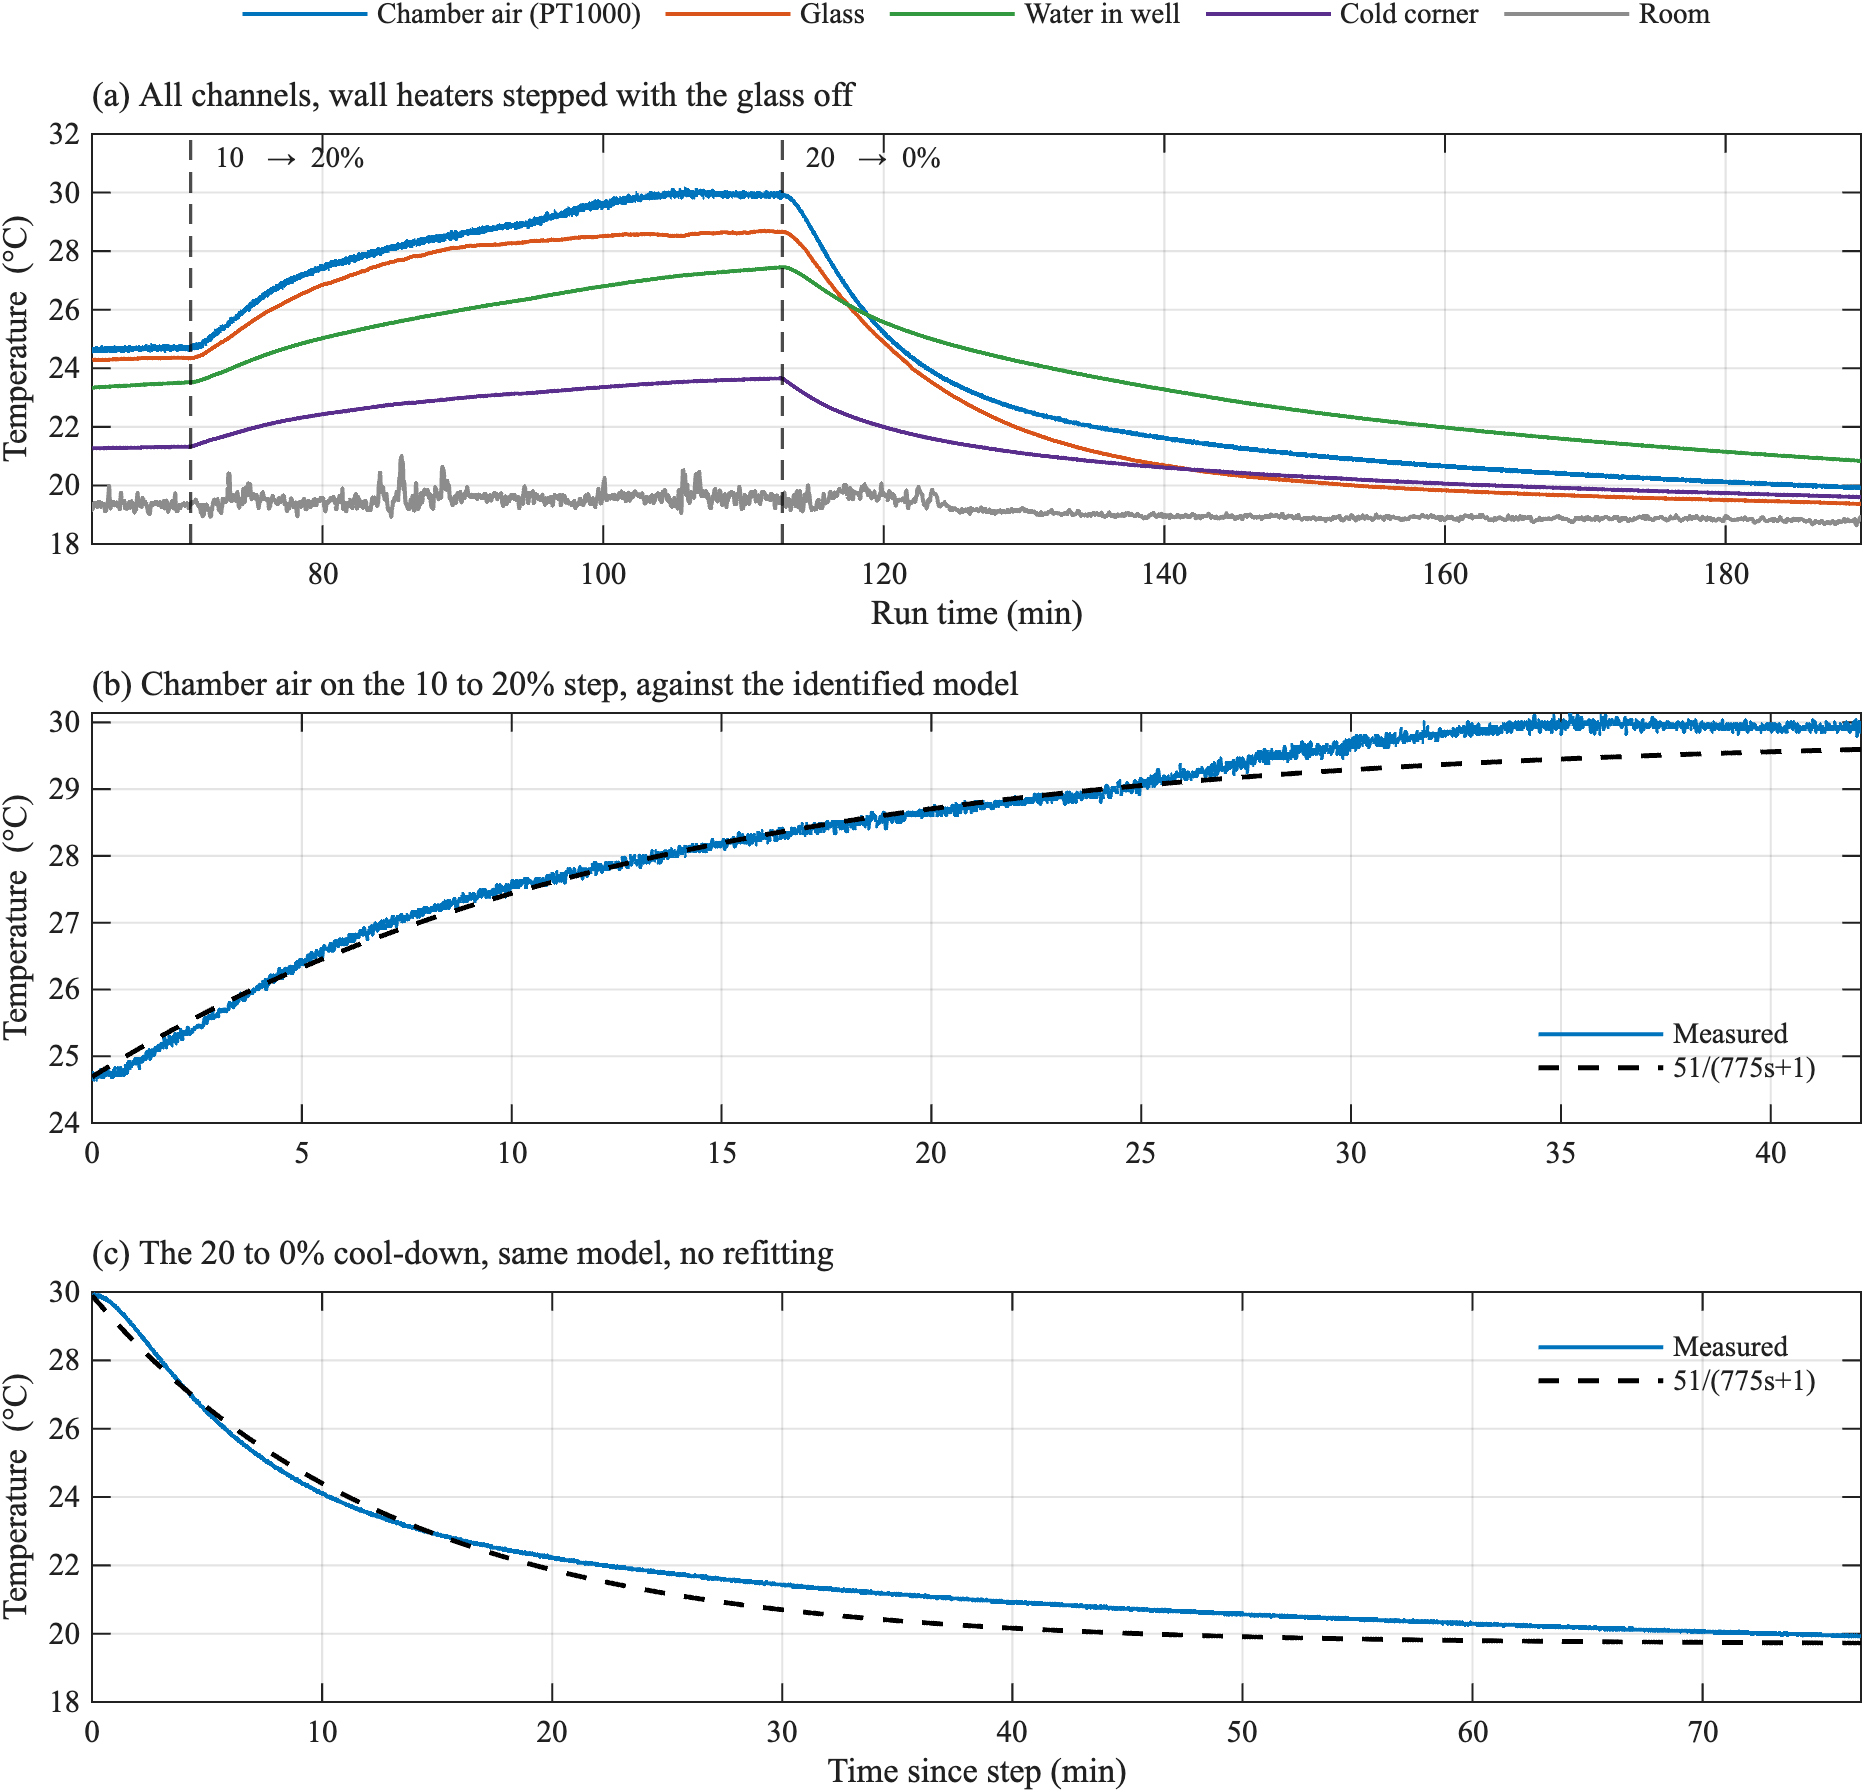
\includegraphics[width=0.58\textwidth]{figs/ch6/fig_T1_heater_step.png}
    \caption[Wall heater step test]{\textbf{Wall heater step test.} (a) All five channels across the run, with the glass held off. (b) The chamber air on the 10 to 20\,\% step, against the model fitted to it. (c) The 20 to 0\,\% cool-down against that same model, with nothing refitted.}
    \label{fig:T1-heater-step}
\end{figure}

Serial logging to file was enabled late, so about 19 minutes covering the cold start and the first step is missing. The 10 to 20\,\% step is still a complete experiment, with a documented steady state, a known input change and a fully logged response, and identifying around an operating point is better practice than identifying from cold. Restarting the monitor does not reset the STM32, and the timestamp runs continuously across it with the duty still at 10\,\%.

Gains are per unit duty, so a 10\,\% step is 0.10. The 10 to 20\,\% step moved the chamber air 5.27\,\textdegree{}C, a gain of 52.7, and switching off from 20\,\% moved it 9.96\,\textdegree{}C, a gain of 49.8. The two agree to 6\,\%, so $K_{11} = 51 \pm 2$. The time constant is less consistent: the two model fits give 760 and 822\,s and the two 63.2\,\% crossings give 801 and 698\,s, averaging 770\,s with a spread of $\pm$62\,s. The model uses 775\,s, giving Equation~\ref{eq:sysid-chamber-tf}. Dead time, the delay while heat crosses the wall and reaches the probe, measured under 30\,s, about 4\,\% of the time constant, and was left out.

\begin{equation}
    G_{11}(s) = \frac{51}{775s + 1}
    \label{eq:sysid-chamber-tf}
\end{equation}

The model tracks the step to within 0.18\,\textdegree{}C, 3\,\% of the 5.27\,\textdegree{}C the chamber moved, and most of that is the room drifting 0.27\,\textdegree{}C during the test. The cool-down in Figure~\ref{fig:T1-heater-step}c is less tidy. Both curves start together and finish within 0.2\,\textdegree{}C, but the measured one falls more slowly in between, sitting up to 0.8\,\textdegree{}C above the model around 36 minutes. The water in the wells and the PETG shell keep releasing heat after the heaters stop and the model has only one store of heat to account for it, with the well still 1.1\,\textdegree{}C above the air an hour later. Logging also stopped 0.19\,\textdegree{}C above the settling point, which is why the cool-down gives the lower of the two gains. None of this affects the controller, which works around a setpoint and never cools from hot to cold.

The glass rose 4.30\,\textdegree{}C on the same step, a cross gain of $K_{21} = 43.0$, so the wall heaters put 84\,\% as much into the glass as into the air. The water in the wells rose 3.88\,\textdegree{}C, a gain of 38.8, so the sample follows 74\,\% of the chamber's response. The rise above room temperature was 5.32\,\textdegree{}C at 10\,\% duty against 10.33\,\textdegree{}C at 20\,\%, a ratio of 1.94 against an ideal 2.00, so the plant is linear over the range the controller will use. Holding 37\,\textdegree{}C in a 20\,\textdegree{}C room needs a 17\,\textdegree{}C rise, which is 33\,\% duty at $K_{11} = 51$, so two heaters hold the setpoint on a third of what they can deliver.

  
 The corner probe sits furthest from either heater, beside the holes where the bulkhead fitting and the cable gland pass through the wall, and the metal in both carries heat straight out to the room. At the 20\,\% plateau it reached only 39\,\% of the way from room to chamber temperature, so at a 37\,\textdegree{}C setpoint it would sit about 10\,\textdegree{}C low. That rules it out as a control location and makes it one of the first places condensate will form. Two limitations apply to the gains: the cable gland was unsealed and the gas line open, so they are lower bounds, and the room drifted 0.27\,\textdegree{}C during the step, which is the main fit error.

\subsection{Model against measurement}
\label{subsec:sysid-chamber-vs-model}

Chapter~\ref{ch:theory} predicted $128/(594s+1)$. The measured plant has 40\,\% of that gain and a 30\,\% longer time constant (Figure~\ref{fig:T3-model-vs-measured}a). Both errors run the same way: the real chamber loses more heat and stores more heat than the model allowed, which is what leaving out the stage, the shell and the penetrations would do. The practical effect is on the duty needed to hold setpoint, predicted at about 9\,\% in a 19\,\textdegree{}C room and measured at 33\,\%. Two heaters still cover that, but with much less spare than the model suggested. A colder room would push the duty higher, and sealing the gland would bring it down. The shape of the response is what the model did get right. The measured plant is first order, stable, with no overshoot and no dead time worth keeping, and a time constant of minutes in both the prediction and the measurement. That is the plant the controller in Section~\ref{sec:control-design} was designed for, so the gains only need recalculating from the measured numbers. A second order or oscillatory plant, or one with a dead time close to $\lambda$, would have meant redesigning the controller.

%*********************************************************************
\section{Lid Glass}
\label{sec:sysid-glass}
%*********************************************************************

\subsection{Step test}
\label{subsec:sysid-glass-test}

The glass was stepped from 0 to 10\,\% at $t = 331$\,s, to 20\,\% at $t = 2913$\,s and off at $t = 5449$\,s, with the wall heaters off throughout. Figure~\ref{fig:T2-glass-step} shows the run. Starting from cold gives two usable 10\,\% steps instead of one. At 0\,\% duty the chamber, glass, corner and room probes read 19.58, 19.46, 19.44 and 19.47\,\textdegree{}C, agreeing to within 0.14\,\textdegree{}C across four sensors and two converters. That independently confirms the calibration in Section~\ref{sec:temperature-commissioning}, on a different day and at a different temperature.

\begin{figure}[htbp]
    \centering
    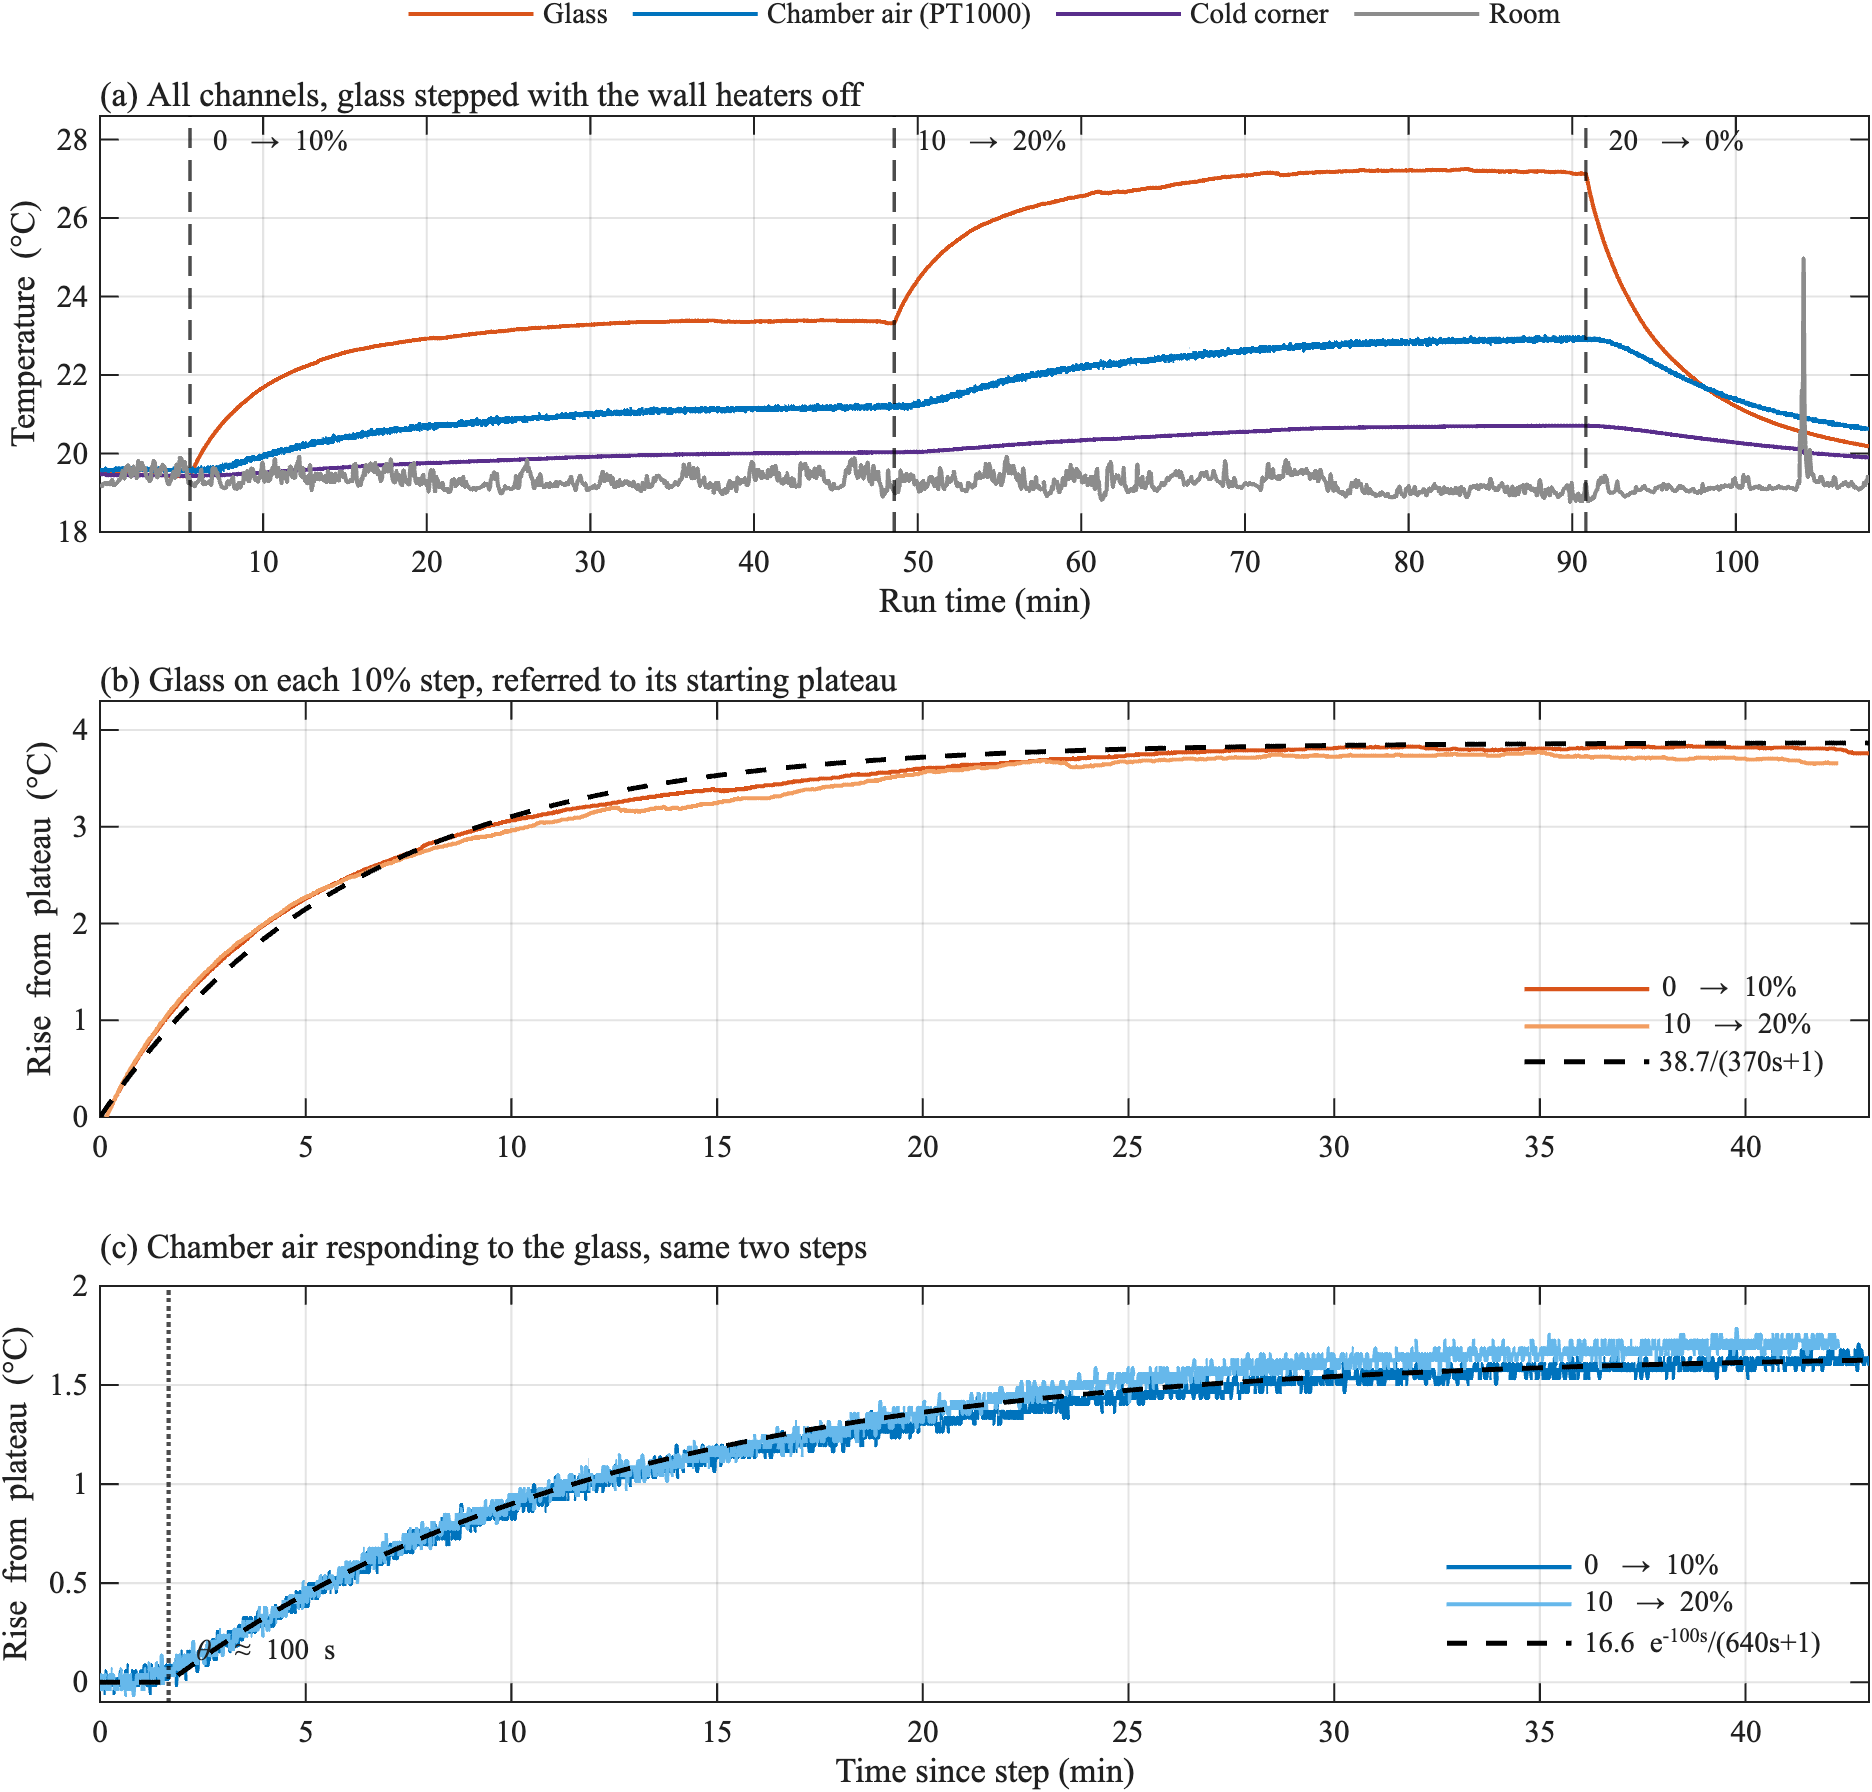
\includegraphics[width=0.56\textwidth]{figs/ch6/fig_T2_glass_step.png}
    \caption[Glass step test]{\textbf{Glass step test.} (a) All four channels across the run, with the wall heaters held off. (b) The glass on each 10\,\% step, each referred to its own starting plateau, against the single model fitted to both. (c) The chamber air responding to the glass on the same two steps, with the transport delay marked. The room probe shows a brief disturbance at 104 minutes, after both steps, where someone passed close to it during the cool-down.}
    \label{fig:T2-glass-step}
\end{figure}



The glass rose 3.92\,\textdegree{}C on the first step and 3.80\,\textdegree{}C on the second, giving gains of 39.2 and 38.0 that agree to 3\,\%. Figure~\ref{fig:T2-glass-step}b shows both steps against the single model fitted to them. The time constant estimates range from 346 to 394\,s, so $\tau_{22} = 370 \pm 25$\,s, giving Equation~\ref{eq:sysid-glass-tf}. The model and the measurement differ by 0.06 to 0.11\,\textdegree{}C, 2 to 3\,\% of the 3.9\,\textdegree{}C step. No dead time could be measured, which is expected for a sensor taped to the element doing the heating.

\begin{equation}
    G_{22}(s) = \frac{38.7}{370s + 1}
    \label{eq:sysid-glass-tf}
\end{equation}

The chamber air responded to the same two steps, giving the cross gain from the glass heater to the air. It rose 1.59 and 1.73\,\textdegree{}C, so $K_{12} = 16.6$, with a time constant of about 640\,s and a dead time of about 100\,s (Figure~\ref{fig:T2-glass-step}c). This dead time is much longer than the under 30\,s of the wall heaters, because the glass has to warm through its own thickness before it can warm the air below.

\subsection{Model against measurement}
\label{subsec:sysid-glass-vs-model}

Chapter~\ref{ch:theory} predicted $73/(158s+1)$. The measured gain is 53\,\% of that and the time constant 2.3 times longer (Figure~\ref{fig:T3-model-vs-measured}b), the same direction and size of error as the chamber's, which points at the same two modelling choices and not at anything specific to the glass.

\begin{figure}[htbp]
    \centering
    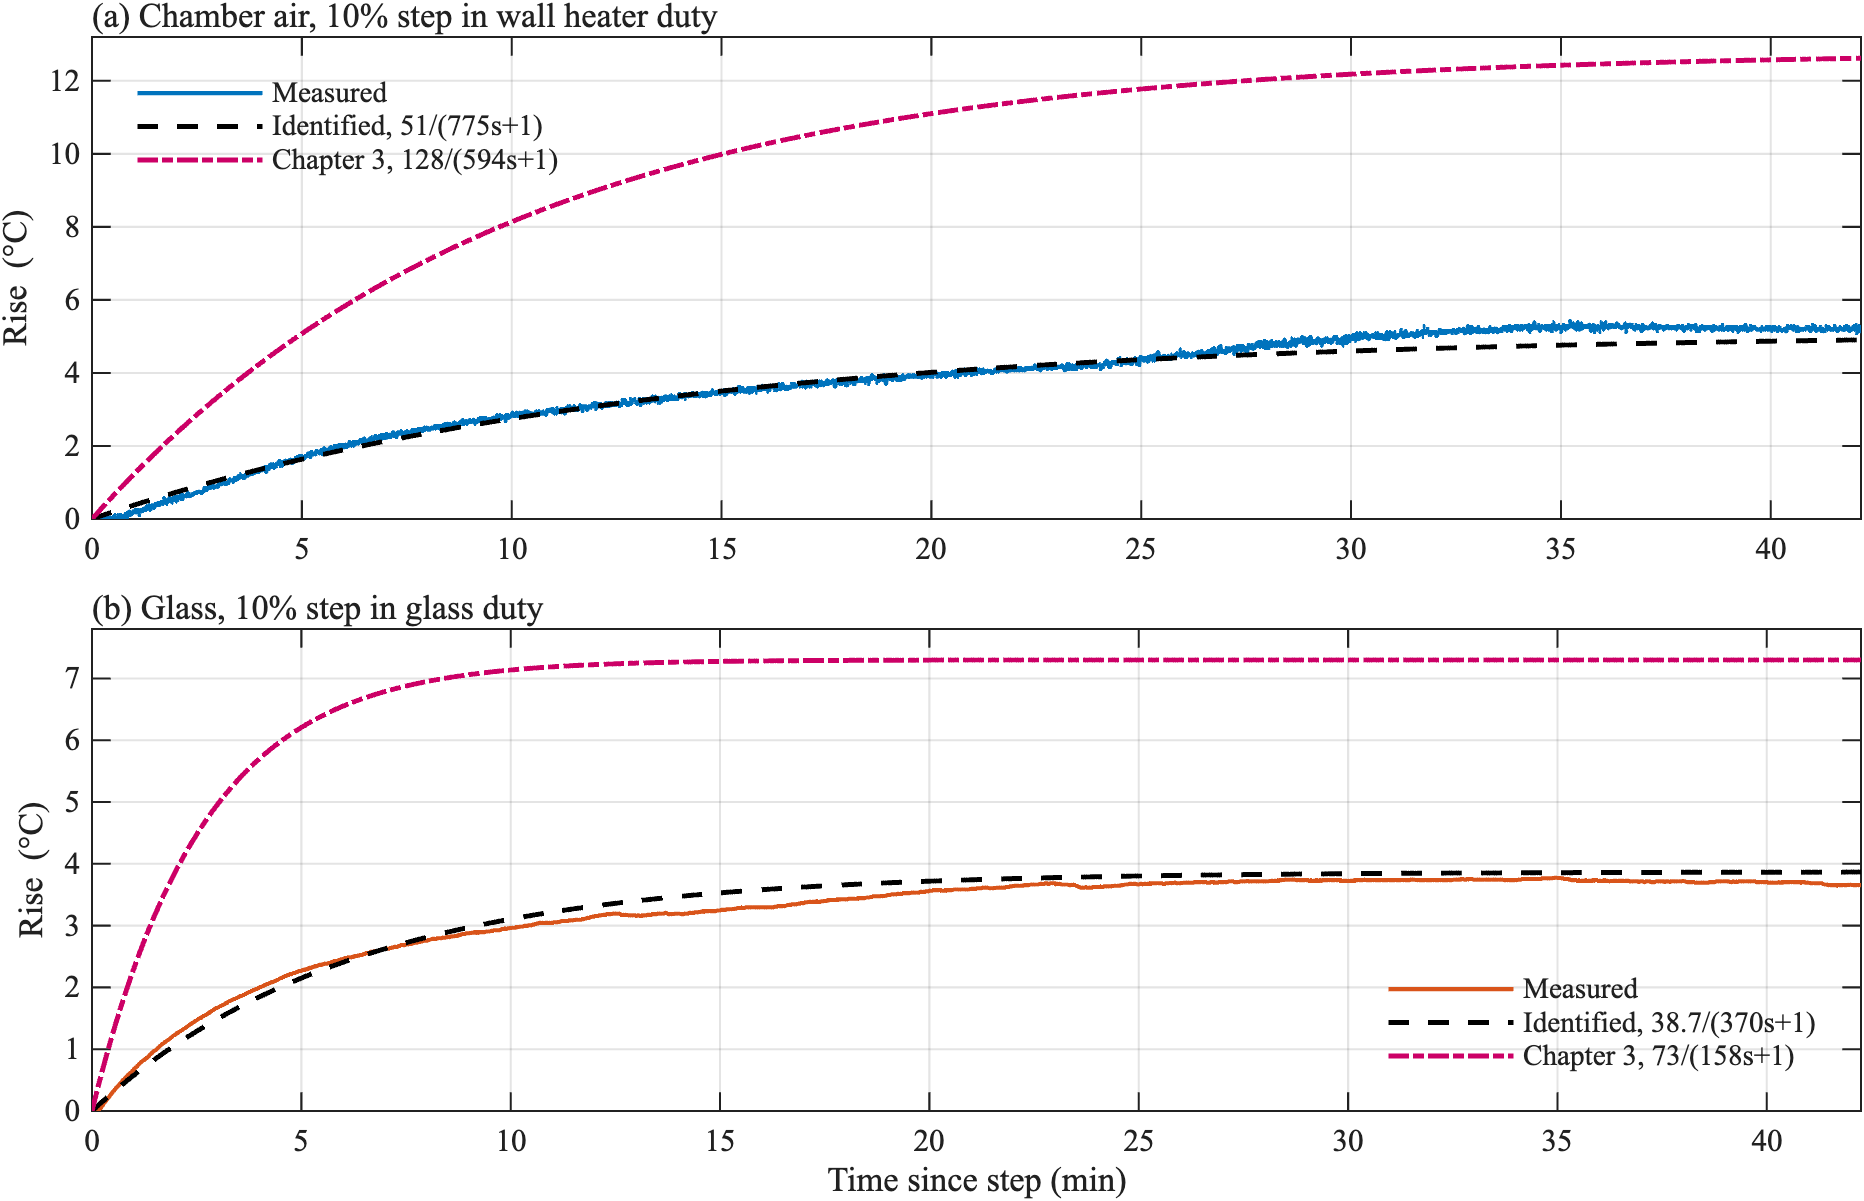
\includegraphics[width=0.60\textwidth]{figs/ch6/fig_T3_model_vs_measured.png}
    \caption[Predicted against measured step response]{\textbf{What Chapter~\ref{ch:theory} predicted against what was measured.} (a) Chamber air on a 10\,\% step in wall heater duty. (b) Glass on a 10\,\% step in glass duty. Both analytical models predict roughly twice the gain of the real plant.}
    \label{fig:T3-model-vs-measured}
\end{figure}

Section~\ref{sec:control-design} argued the two loops could be designed separately, since independent PI loops are only valid when one settles before the other has moved. That argument used the plant time constants, with the glass about four times faster than the chamber. Measured, the glass is 370\,s against the chamber's 775\,s, only about twice as fast, so that argument is weaker than it looked. The design does not depend on it. The loops run at the closed loop speeds, $\lambda = 60$\,s for the glass against 300\,s for the chamber, a factor of five. Identifying the plant changes $K$ and $\tau$. It does not change $\lambda$. The pairing is also still correct, since each heater affects its own temperature more than the other. The measurements do change the gain the chamber loop sees, and that is the subject of the next section.

%*********************************************************************
\section{Updated Controller Gains}
\label{sec:sysid-gains}
%*********************************************************************

The two step tests give the four steady state gains of Equation~\ref{eq:sysid-gain-matrix}, in \textdegree{}C per unit duty. The inputs are the wall heater and glass duties, and the outputs are the chamber air and glass temperatures.

\begin{equation}
    K =
    \begin{bmatrix}
        K_{11} & K_{12} \\
        K_{21} & K_{22}
    \end{bmatrix}
    =
    \begin{bmatrix}
        51.0 & 16.6 \\
        43.0 & 38.7
    \end{bmatrix},
    \qquad
    \begin{array}{ll}
        K_{11}: & \text{wall heater} \rightarrow \text{chamber air} \\
        K_{12}: & \text{glass heater} \rightarrow \text{chamber air} \\
        K_{21}: & \text{wall heater} \rightarrow \text{glass} \\
        K_{22}: & \text{glass heater} \rightarrow \text{glass}
    \end{array}
    \label{eq:sysid-gain-matrix}
\end{equation}

The off-diagonal terms are large. $K_{21} = 43.0$ means the wall heaters heat the glass almost as much as they heat the air, so turning them up is also a disturbance to the glass loop. The glass loop is the faster of the two and reacts straight away, cutting its own heating, so the glass delivers less heat into the chamber than before.

Take the wall heaters up by one unit of duty. The glass rises by 43.0\,\textdegree{}C. One unit of glass duty raises the glass by $K_{22} = 38.7$\,\textdegree{}C, so the glass loop cuts its own duty by $43.0/38.7 = 1.11$ units to bring the glass back to setpoint. Each unit of glass duty is also worth $K_{12} = 16.6$\,\textdegree{}C to the chamber air, so cutting 1.11 units costs the chamber 18.4\,\textdegree{}C of heating. The chamber ends up 32.6\,\textdegree{}C warmer, not 51.

\begin{equation}
    K_\mathrm{eff} = K_{11} - \frac{K_{12}K_{21}}{K_{22}} = 51 - \frac{16.6 \times 43.0}{38.7} = 32.6.
    \label{eq:sysid-keff}
\end{equation}

So $K_\mathrm{eff} = 32.6$ from Equation~\ref{eq:sysid-keff} replaces $K_{11} = 51$ as the gain the chamber controller is tuned against. The glass gain is left alone, since the chamber loop is too slow to react to the glass the same way. Tuning the chamber against 51 would make $K_p$ 1.6 times too small and the loop 1.6 times slower than designed. Both sets of gains are recalculated from Equation~\ref{eq:lambda-gains} with nothing else changed (Table~\ref{tab:sysid-gains}): same PI structure, same lambda tuning, same $\lambda$, setpoint weight and sample time. The correction holds only while the glass loop is running. With the glass loop off or saturated, the chamber sees 51 again and its proportional gain is 1.6 times more aggressive than intended.

\begin{table}[htbp]
    \centering
    \caption{Controller gains before and after identification. Values are per unit duty; multiply by 100 for percent duty.}
    \label{tab:sysid-gains}
    \small
    \begin{tabular}{llccccc}
        \toprule
        \textbf{Loop} & \textbf{Source} & $K$ & $\tau$ & $\lambda$ & $K_p$ & $K_i$ \\
        \midrule
        Chamber & Chapter~\ref{ch:theory} & 128 & 594\,s & 300\,s & 0.0155 & $2.60\times10^{-5}$ \\
        Chamber & Measured & 32.6 & 775\,s & 300\,s & \textbf{0.0790} & $\mathbf{1.02\times10^{-4}}$ \\
        \midrule
        Glass & Chapter~\ref{ch:theory} & 73 & 158\,s & 60\,s & 0.0361 & $2.28\times10^{-4}$ \\
        Glass & Measured & 38.7 & 370\,s & 60\,s & \textbf{0.159} & $\mathbf{4.31\times10^{-4}}$ \\
        \bottomrule
    \end{tabular}
\end{table}

The chamber proportional gain rises five times and the glass four. The integral times become $T_i = \tau$, 775\,s for the chamber and 370\,s for the glass. Both loops stay well inside the duty range, since 33\,\% holds 37\,\textdegree{}C and the error that would saturate the chamber loop on proportional action alone is $1/K_p = 12.7$\,\textdegree{}C.

%*********************************************************************
\section{Summary}
\label{sec:sysid-summary}
%*********************************************************************

Both loops are now identified from the built chamber, $51/(775s+1)$ and $38.7/(370s+1)$. Two limits apply to what follows: the gland was unsealed and the gas line open, so the gains are lower bounds on the sealed chamber; and both loops were identified around 25 to 30\,\textdegree{}C, so the closed loop results are the first test of whether these parameters hold at 37\,\textdegree{}C.

%*********************************************************************
% End of Thermal System Identification
%*********************************************************************